%%%%%%%%%%%%%%%%%%%%%%%%%%%%%%%%%%%%%%%%%
%
% CMPT 435
% Lab Zero
%
%%%%%%%%%%%%%%%%%%%%%%%%%%%%%%%%%%%%%%%%%

%%%%%%%%%%%%%%%%%%%%%%%%%%%%%%%%%%%%%%%%%
% Short Sectioned Assignment
% LaTeX Template
% Version 1.0 (5/5/12)
%
% This template has been downloaded from: http://www.LaTeXTemplates.com
% Original author: % Frits Wenneker (http://www.howtotex.com)
% License: CC BY-NC-SA 3.0 (http://creativecommons.org/licenses/by-nc-sa/3.0/)
% Modified by Alan G. Labouseur  - alan@labouseur.com, and Patrick Tyler - Patrick.Tyler1@marist.edu
%
%%%%%%%%%%%%%%%%%%%%%%%%%%%%%%%%%%%%%%%%%

%----------------------------------------------------------------------------------------
%	PACKAGES AND OTHER DOCUMENT CONFIGURATIONS
%----------------------------------------------------------------------------------------

\documentclass[letterpaper, 10pt]{article} 

\usepackage[english]{babel} % English language/hyphenation
\usepackage{graphicx}
\usepackage[lined,linesnumbered,commentsnumbered]{algorithm2e}
\usepackage{listings}
\usepackage{fancyhdr} % Custom headers and footers
\pagestyle{fancyplain} % Makes all pages in the document conform to the custom headers and footers
\usepackage{lastpage}
\usepackage{xcolor}
\usepackage{url}
\usepackage{titlesec}

% Stolen from https://www.overleaf.com/learn/latex/Code_listing 
\definecolor{codegreen}{rgb}{0,0.6,0}
\definecolor{codegray}{rgb}{0.5,0.5,0.5}
\definecolor{codepurple}{rgb}{0.58,0,0.82}
\definecolor{backcolour}{rgb}{0.95,0.95,0.92}

\lstdefinestyle{mystyle}{
    backgroundcolor=\color{backcolour},   
    commentstyle=\color{codegreen},
    keywordstyle=\color{magenta},
    numberstyle=\tiny\color{codegray},
    stringstyle=\color{codepurple},
    basicstyle=\ttfamily\footnotesize,
    breakatwhitespace=false,         
    breaklines=true,                 
    captionpos=b,                    
    keepspaces=true,                 
    numbers=left,                    
    numbersep=5pt,                  
    showspaces=false,                
    showstringspaces=false,
    showtabs=false,                  
    tabsize=2
}
\lstset{style=mystyle, language=c++}


\fancyhead{} % No page header - if you want one, create it in the same way as the footers below
\fancyfoot[L]{} % Empty left footer
\fancyfoot[C]{page \thepage\ of \pageref{LastPage}} % Page numbering for center footer
\fancyfoot[R]{}

\renewcommand{\headrulewidth}{0pt} % Remove header underlines
\renewcommand{\footrulewidth}{0pt} % Remove footer underlines
\setlength{\headheight}{13.6pt} % Customize the height of the header

%----------------------------------------------------------------------------------------
%	TITLE SECTION
%----------------------------------------------------------------------------------------

\newcommand{\horrule}[1]{\rule{\linewidth}{#1}} % Create horizontal rule command with 1 argument of height

\title{	
   \normalfont \normalsize 
   \textsc{CMPT 435 - Fall 2023 - Dr. Labouseur} \\[10pt] % Header stuff.
   \horrule{0.5pt} \\[0.25cm] 	% Top horizontal rule
   \huge Assignment Four -- \LaTeX ~DP and Greedy\\     	    % Assignment title
   \horrule{0.5pt} \\[0.25cm] 	% Bottom horizontal rule
}

\author{Patrick Tyler \\ \normalsize Patrick.Tyler1@marist.edu}

\date{\normalsize\today} 	% Today's date.

\begin{document}
\maketitle % Print the title
\section{Dynamic Programming}
Dynamic programming (DP) is the computer science technique of using results from a previous calculation
is the rest of the program (breaking problems into smaller pieces). This is useful when you have expensive pure functions 
which by definition is a function which returns the same value for the same input and has no side effects.
A popular problem which benefits heavily from a DP approach is calculating
the fibonacci sequence recursively. There is a lot of identical calls when calculating the fibonacci sequence.
So, if the results are cached a lot of computation can be saved as demonstrated in figure 1.
\begin{figure}[h]
    \centering
    % source: https://avikdas.com/2019/04/15/a-graphical-introduction-to-dynamic-programming.html
    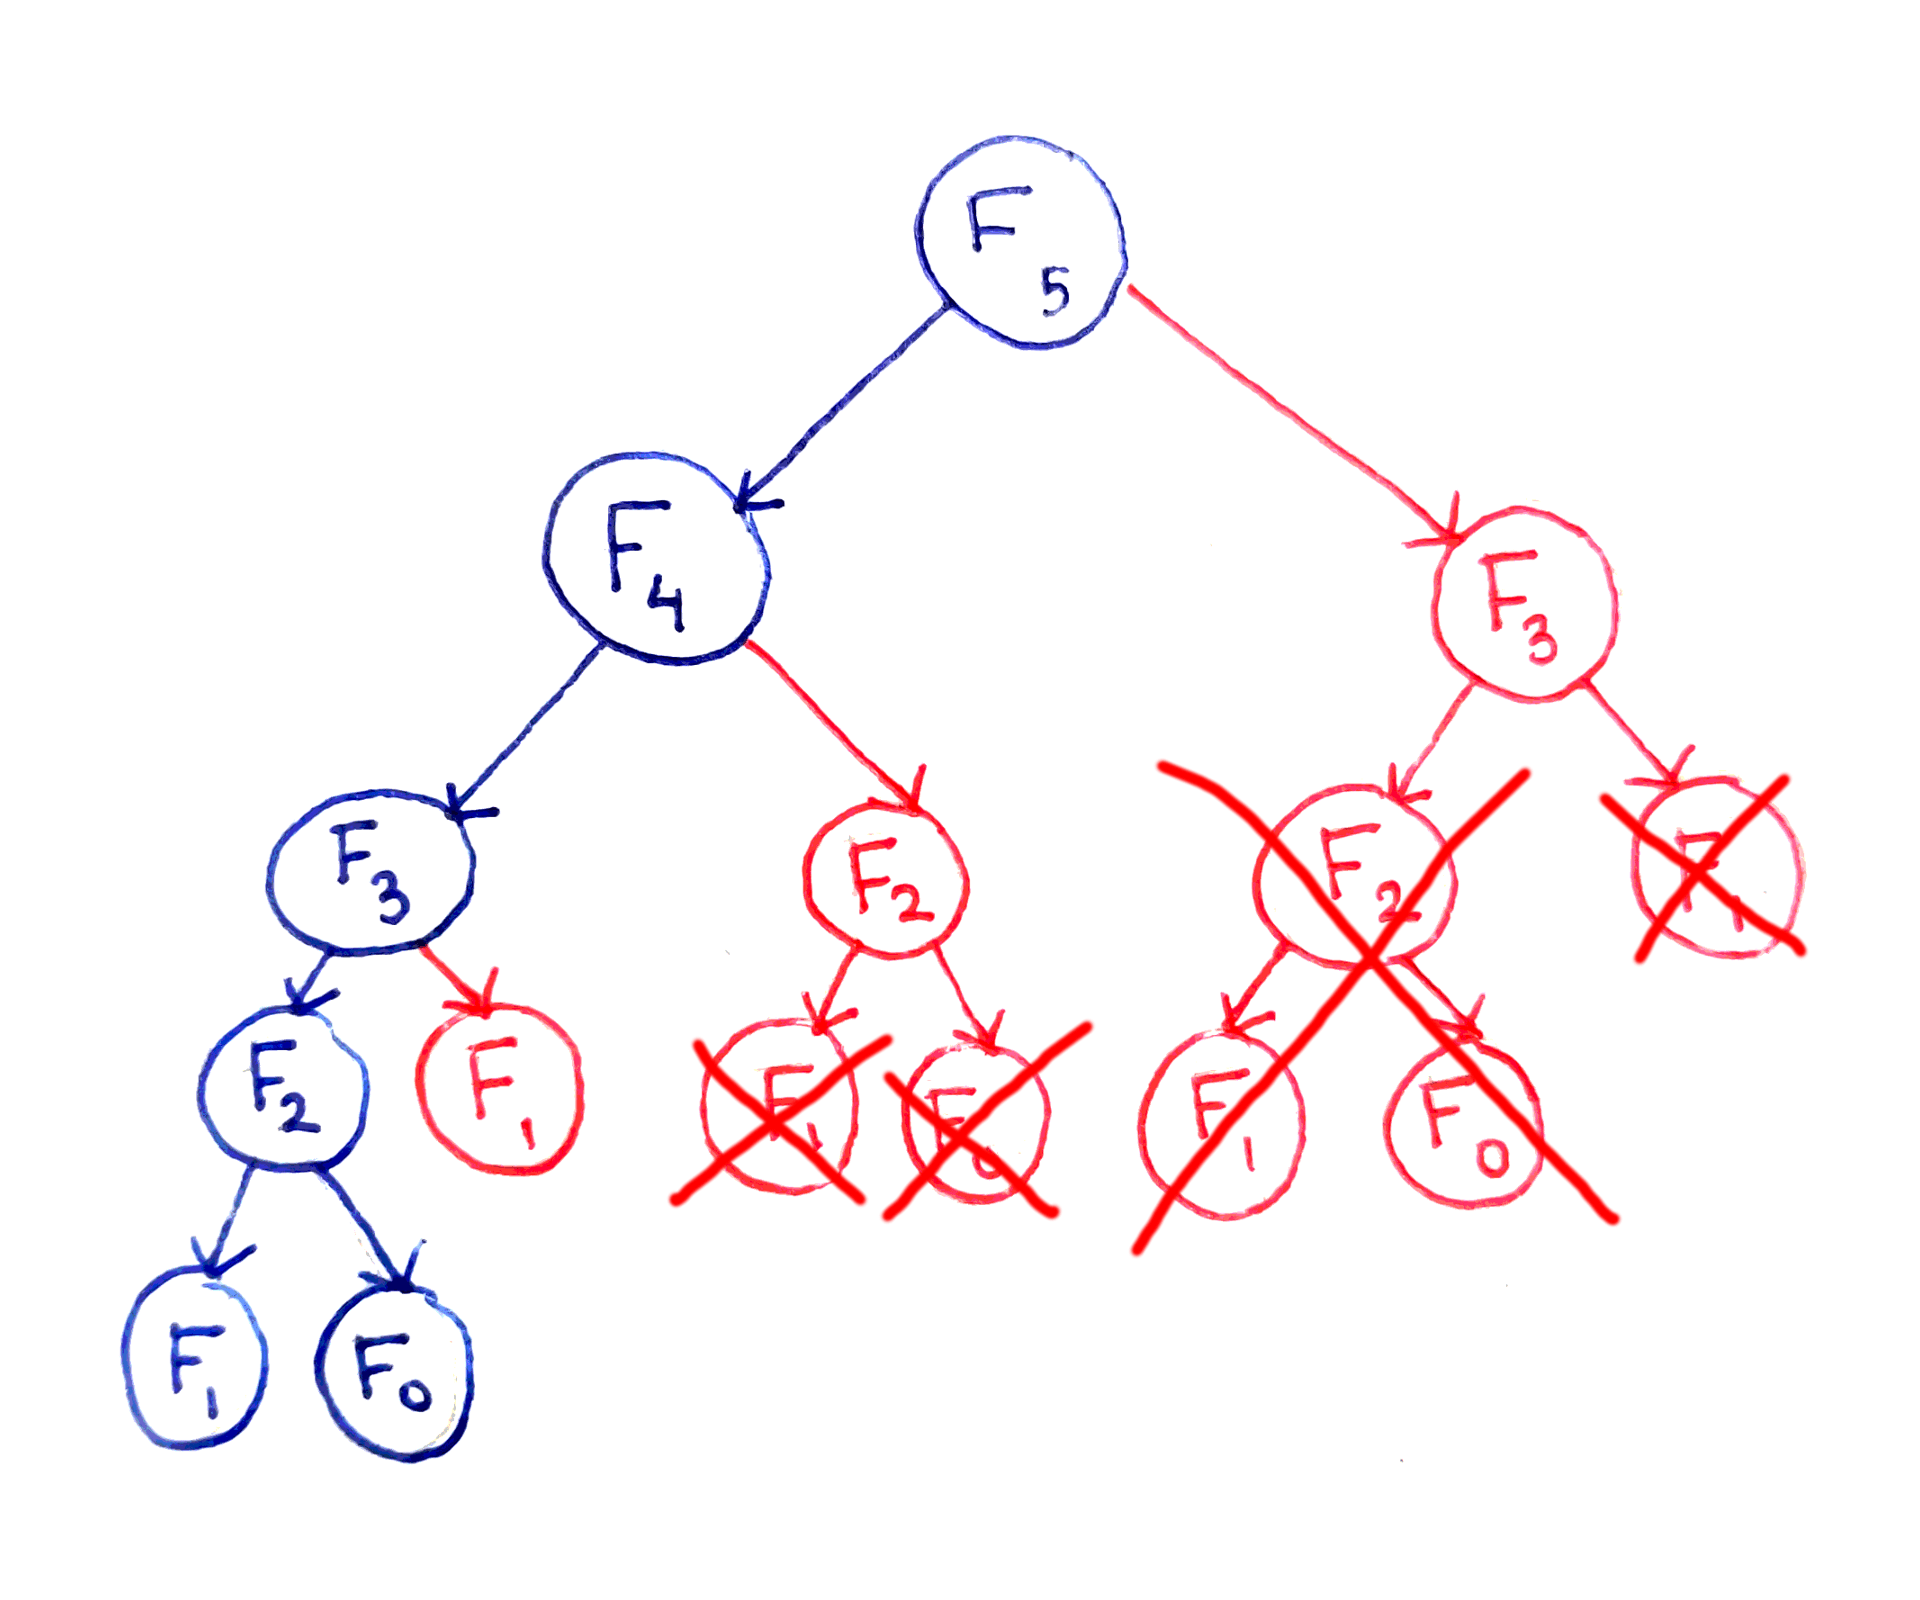
\includegraphics[width=.5\textwidth]{fibonacci-memoized.png}
    \caption{Fibonacci Sequence from Avik Das}
    \label{fig:your_label}
\end{figure}
\newpage
\subsection{Bellman Ford Algorithm}
Another algorithm which takes advantage of DP is the Bellman Ford algorithm. This algorithm finds the shortest distances
from a source vertex to the other reachable vertices in a weighted graph. The steps of this algorithm are as follows:\\
1. Initialize storage of current distance values and predecessors. The starting distance from starting vertex
should always compare as greater than a finite distance so infinity is used. The distance from the starting vertex
to itself is 0.
\lstinputlisting[linerange={244-249}, firstnumber=244]{main.cpp}
2. For each edge check where u is the \textbf{from} vertex, v is the \textbf{to}, and its distance is defined
as the stored shortest path from the starting point. Check if u's distance plus the edge weight is less than v'sa
current weight. If it that check is true then update the distance with the shortest value and v's predecessor to u.
The checking and updating process is generally referred to as "relaxing" the edge.
\lstinputlisting[linerange={254-268}, firstnumber=254]{main.cpp}
3. Repeat 2. till is has been completed one less than the count of vertices. This insures that the algorithm has
enough iterations to propagate the distance values at most the count of vertices minus 1. This should be intuitive
because any given edge can be a most vertices count minus 1 edges away from the starting vertex if it is reachable at all.
\\
4. Check for any negative edge cycles. If one of these exists then the minimum path is indefinitely small / negative
infinity.
\lstinputlisting[linerange={272-287}, firstnumber=272]{main.cpp}
\end{document}

